\section{Concurrency Control}

\paragraph{Transaction}
\begin{itemize}
\item Reliable unit of work against memory abstraction
\end{itemize}

\paragraph{ACID Properties}
\begin{itemize}
\item \textbf{Atomicity:} transactions are all-or-nothing
\item \textbf{Consistency:} transaction takes database from
  one consistent state to another
\item \textbf{Isolation:} Executes as if it were the only one in
  the systems (aka before-or-after atomicity)
\item \textbf{Durability:} once transaction is done (``committed''),
  results are persistent in the database
\end{itemize}

\paragraph{The many faces of atomicity}
\begin{itemize}
\item \textbf{Atomicity} is strong modularity mechanism!
  \begin{itemize}
  \item Hides that one high-level actions is actually made of
    many sub-actions
  \end{itemize}

\item \textbf{Before-or-after} atomicity
  \begin{itemize}
  \item == Isolation
  \item Cannot have effects that would only arise by
    interleaving of parts of transactions
  \end{itemize}

\item \textbf{All-or-nothing} atomicity
  \begin{itemize}
  \item == Atomicity (+ Durability)
  \item cannot have partially executed transactions
  \item Once executed and confirmed, transaction effects are
    visible and not forgotten
  \end{itemize}
\end{itemize}

\paragraph{Goal of Concurrency Control}
\begin{itemize}
\item Transactions should be executed so that it is
  \textit{as though} they executed in some serial order
  \begin{itemize}
  \item Also called \textbf{Isolation} or \textbf{Serializability}
    or \textbf{Before-or-after atomicity}
  \end{itemize}

\item Weaker variants also possible
  \begin{itemize}
  \item Lower ``degrees of isolation''
  \end{itemize}
\end{itemize}

\paragraph{Example}
Consider two transactions (Xacts):

\begin{lstlisting}
  T1: BEGIN A=A+100, B=B-100 END
  T2: BEGIN A=1.06*A, B=1.06*B END
\end{lstlisting}

\begin{itemize}
\item T1 transfers \$100 from B's account to A's account
\item T2 credits both accounts with 6\% interest
\item If submitted concurrently, net effect should be equivalent
  to Xacts running in some serial order
  \begin{itemize}
  \item No guarantee that T1 ``logically'' occurs before T2
    (or vice-versa) - but one of them is true
  \end{itemize}
\end{itemize}

\paragraph{Different Solutions (Locking Protocols)}

\paragraph{Solution 1}

\begin{enumerate}
\item Get exclusive lock on entire database
\item Execute transaction
\item Release exclusive lock
\end{enumerate}

\begin{itemize}
\item Transactions execute in \textit{critical section}
\item Serializability guaranteed because execution is serial!
\end{itemize}

\textbf{{\color{red} Problems:}}
\begin{itemize}
\item no concurrency, only serial schedules
\end{itemize}

\paragraph{Solution 2}
\begin{enumerate}
\item Get exclusive locks on \textit{accessed} data items
\item execute transaction
\item release exclusive locks
\end{enumerate}

\begin{itemize}
\item Greater concurrency
\end{itemize}

\textbf{{\color{red} Problems:}}
\begin{itemize}
\item need to know objects a priori, least concurrency
\end{itemize}

\paragraph{Solution 3}
\begin{enumerate}
\item Get exclusive locks on data items that are
  \textit{modified}; get shared locks on data items that
  are only \textit{read}
\item Execute transaction
\item Release all locks
\end{enumerate}

\begin{itemize}
\item Greater concurrency
\item Conservative Strict Two Phase Locking (CS2PL)
\end{itemize}

\textbf{{\color{red} Problems:}}
\begin{itemize}
\item need to know objects a priori, least concurrency
\end{itemize}

\paragraph{Solution 4}
\begin{enumerate}
\item Get exclusive locks on data items that are modified and get
  shared locks on data items that are read
\item Execute transaction and release locks on objects
  no longer needed \textit{during execution}
\end{enumerate}

\begin{itemize}
\item Greater concurrency
\item Conservative Two Phase Locking (C2PL)
\end{itemize}

\textbf{{\color{red} Problems:}}
\begin{itemize}
\item Cascading Aborts: assume T1 has locks on $1,2,3$ and
  then starts to release locks $1,2$, which are immediately
  acquired by T2, but then T1 does not commit but aborts.
  now T2 also has to be aborted etc.
\item need to know objects a priori, when to release locks
\end{itemize}


\paragraph{Solution 5}
\begin{enumerate}
\item Get exclusive locks on data items that are modified and
  get shared locks on data items that are read, but do this
  \textit{during execution} of transaction (as needed)
\item Release all locks
\end{enumerate}

\begin{itemize}
\item Greater concurrency
\item Strict Two Phase Locking (S2PL)
\end{itemize}

\textbf{{\color{red} Problems:}}
\begin{itemize}
\item Deadlocks: assume T1 wants $1,2,3$ and T2 wants $2,3,4$
  and that T1 acquires $1,2$ and T2 $3,4$ now we have a deadlock.
\end{itemize}


\paragraph{Solution 6}
\begin{enumerate}
\item Get exclusive locks on data items that are modified and get
  shared locks on data items that are read, but do this during execution
  of transaction (as needed)
\item Release locks on objects no longer needed during execution
  of transaction
\item Cannot acquire locks once any lock has been released
  (Hence two-phase (acquiring phase and releasing phase)
\end{enumerate}

\begin{itemize}
\item Greater concurrency
\item Two Phase Locking (2PL)
\end{itemize}

\textbf{{\color{red} Problems:}}
\begin{itemize}
\item Cascading aborts and Deadlocks
\end{itemize}

\paragraph{Summary of Alternatives}
\begin{itemize}
\item Conservative Strict 2PL
  \begin{itemize}
  \item no deadlocks, no cascading aborts
  \item \textbf{But} need to know objects a priori, least concurrency
  \end{itemize}
\begin{figure}[h]
  \begin{minipage}{1.0\linewidth}
    \begin{center}
      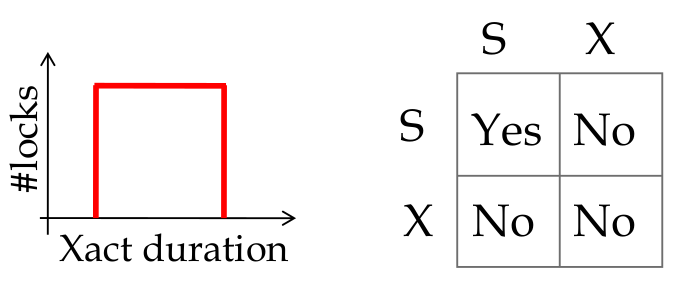
\includegraphics[scale=0.15]{graphics/CS2PL.png}
    \end{center}
  \end{minipage}
\end{figure}

\item Conservative 2PL
  \begin{itemize}
  \item no deadlocks, more concurrency than Conservative Strict 2PL
  \item \textbf{But} need to know objects a priori, when to
    release locks, need to deal with cascading aborts
  \end{itemize}
\begin{figure}[h]
  \begin{minipage}{1.0\linewidth}
    \begin{center}
      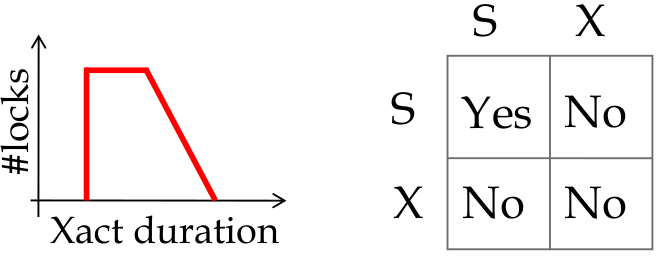
\includegraphics[scale=0.15]{graphics/C2PL.png}
    \end{center}
  \end{minipage}
\end{figure}



\item Strict 2PL
  \begin{itemize}
  \item no cascading aborts, no need to know objects a priori or
    when to release locks, more concurrency than
    Conservative Strict 2PL
  \item \textbf{But} deadlocks
  \end{itemize}
\begin{figure}[h]
  \begin{minipage}{1.0\linewidth}
    \begin{center}
      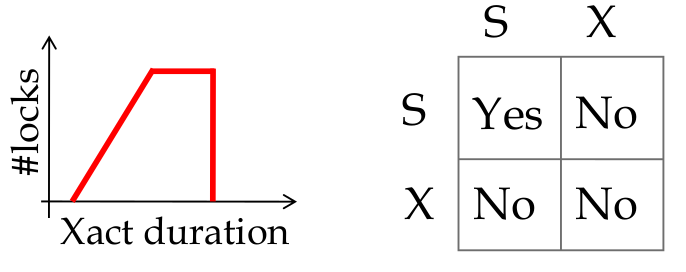
\includegraphics[scale=0.15]{graphics/S2PL.png}
    \end{center}
  \end{minipage}
\end{figure}

\vspace{1.5cm}
\item 2PL
  \begin{itemize}
  \item most concurrency, no need to know objects a priori
  \item \textbf{But} need to know when to release locks,
    cascading aborts, deadlocks
  \end{itemize}
\begin{figure}[h]
  \begin{minipage}{1.0\linewidth}
    \begin{center}
      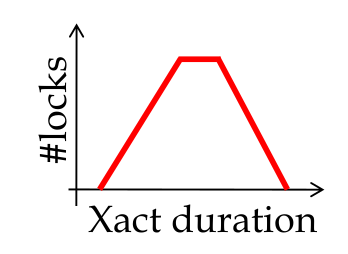
\includegraphics[scale=0.15]{graphics/2PL.png}
    \end{center}
  \end{minipage}
\end{figure}
\end{itemize}

\paragraph{Method of choice}
\begin{itemize}
\item Strict 2PL
  \begin{itemize}
  \item no cascading aborts, no need to know objects a priori or
    when to release locks, more concurrency than Conservative
    Strict 2PL
  \item But deadlocks
  \end{itemize}

\item Reason for choice
  \begin{itemize}
  \item Cannot know objects a priori, so no Conservative options
    → only if you would know something about application!
  \item Thus only 2PL and Strict 2PL left
  \item 2PL needs to know when to release locks (main problem),
    and has cascading aborts
  \item Hence Strict 2PL
  \end{itemize}

\item Implication: Need to deal with deadlocks!
\end{itemize}


\paragraph{Lock Management}
\begin{itemize}
\item Lock/unlock requests handled by lock manager

\item Lock table entry:
  \begin{itemize}
  \item Number of transactions currently holding a lock
  \item Type of lock held (shared or exclusive)
  \item Pointer to queue of lock requests
  \end{itemize}

\item Locking and unlocking have to be atomic operations

\item \textbf{Lock upgrade:} transaction that holds a shared lock
  can be upgraded to hold an exclusive lock
\end{itemize}


\paragraph{Dynamic Databases: Locking the objects that exist
  now in the database is not enough!}
\begin{itemize}
\item If we relax the assumption that the DB is a fixed collection
  of objects, even Strict 2PL will not work correctly:
  \begin{itemize}
  \item T1 locks all pages containing sailor records with
    \textit{rating} = 1, and finds \textbf{oldest} sailor (say, age = 71)
  \item Next, T2 inserts a new sailor; rating = 1, age = 96
  \item T2 also deletes oldest sailor with rating = 2 (and, say,
    age = 80), and commits
  \item T1 now locks all pages containing sailor records with
    rating = 2, and finds \textbf{oldest} (say, age = 63)
  \end{itemize}

\item No consistent DB state where T1 is ``correct''!
\end{itemize}

\paragraph{The Problem}
\begin{itemize}
\item T1 implicitly assumes that it has locked the set of all
  sailor records with rating = 1
  \begin{itemize}
  \item assumption only holds if no sailor records are added while
    T1 is executing!
  \item Need some mechanism to enforce this assumption.
    \textbf{(Index locking and predicate locking)}
  \end{itemize}

\item Example shows that correctness is guaranteed for locking on
  individual objects only if the set of objects is fixed!
\end{itemize}


\paragraph{Index Locking}
\begin{itemize}
\item If data is accessed by an \textbf{index} on the rating field,
  T1 should \textbf{lock the index page} containing the data entries
  with rating = 1
  \begin{itemize}
  \item if there are no records with rating = 1, T1 must lock the
    index page where such a data entry would be, if it existed!
  \end{itemize}

\item if there is \textbf{no suitable index}, T1 must
  \textbf{lock all pages}, and lock the file/table to prevent new
  pages from being added, to ensure that no new records
  with rating = 1 are added
\end{itemize}

\paragraph{Multiple-Granularity Locks}
\begin{itemize}
\item Hard to decide what granularity to lock
  (tuple vs. pages vs. tables)
\item Shouldn't have to decide!
\item Data ``containers'' are nested
\end{itemize}
\begin{figure}[h]
  \begin{minipage}{1.0\linewidth}
    \begin{center}
      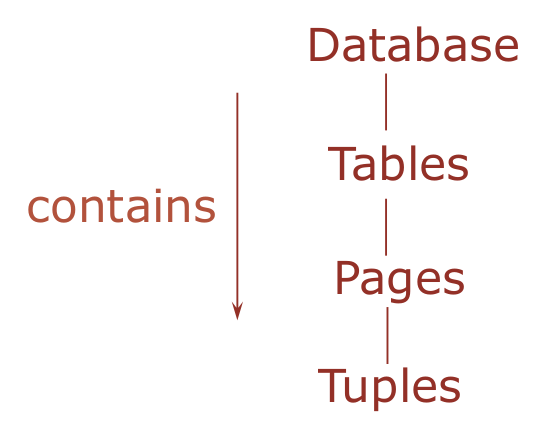
\includegraphics[scale=0.15]{graphics/DB_granularity.png}
    \end{center}
  \end{minipage}
\end{figure}


\paragraph{Solution: New Lock Modes, Protocol}

\begin{minipage}{0.3\textwidth}
  \begin{itemize}
  \item Allow Xacts to lock at each level, but with a
    special protocol using new \textbf{``intention'' locks}
  \item before locking and item, Xact must set ``intention locks''
    on all its ancestors
  \item for unlock, go from specific to general
    (i.e., bottom-up)
  \item \textbf{SIX mode:} like S \& IX at the same time
  \end{itemize}
\end{minipage}%
\begin{minipage}{0.5\textwidth}
  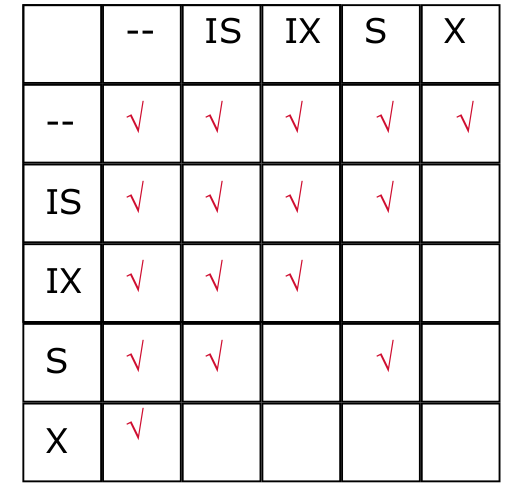
\includegraphics[scale=0.15]{graphics/intention-locks.png}
\end{minipage}


\paragraph{Schedules}
\begin{itemize}
\item Consider a possible interleaving (schedule):

  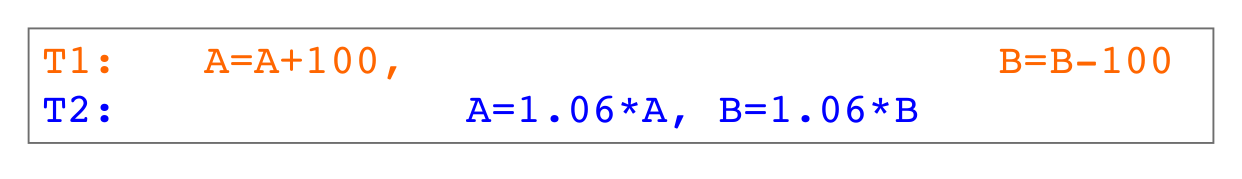
\includegraphics[scale=0.15]{graphics/schedule-1.png}

\item The systems's view of the schedule

  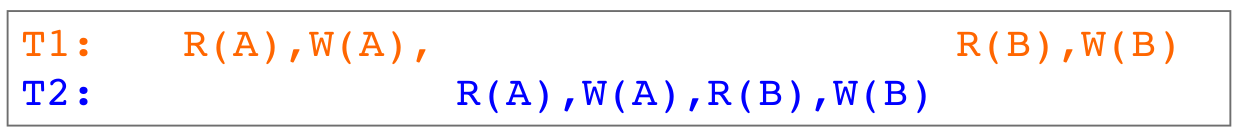
\includegraphics[scale=0.15]{graphics/schedule-2.png}
\end{itemize}

\paragraph{Scheduling Transactions}
\begin{itemize}
\item \textbf{Serial schedule:} Schedule that does not
  interleave the actions of different transactions


\item \textbf{Equivalent schedules:} For any database state
  \begin{itemize}
  \item The effect (on the set of objects in the database) of
    executing the schedules is the same
  \item the values read by transactions is the same in the
    schedules
    \begin{itemize}
    \item Assume no knowledge of transaction logic
    \end{itemize}
  \end{itemize}

\item \textbf{Serializable schedule:} A schedule that is equivalent
  to some serial execution of the transactions.
\end{itemize}

\paragraph{Anomalies with Interleaved Execution}
\begin{itemize}
\item Reading Uncommitted Data (WR Conflicts, ``dirty reads'')

  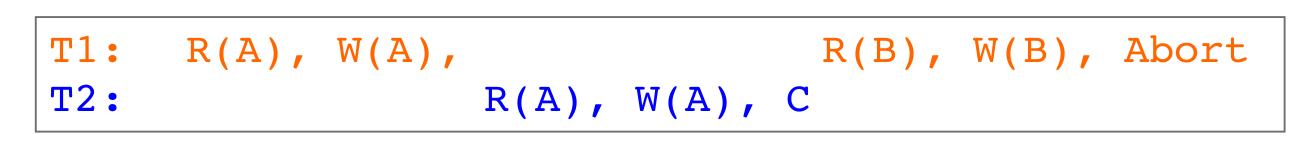
\includegraphics[scale=0.15]{graphics/WR-conflicts.png}

\item Unrepeatable Reads (RW Conflicts)

  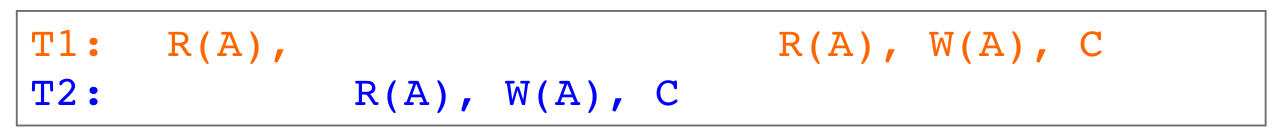
\includegraphics[scale=0.15]{graphics/RW-conflicts.png}

\item Overwriting Uncommitted Data (WW Conflicts)

  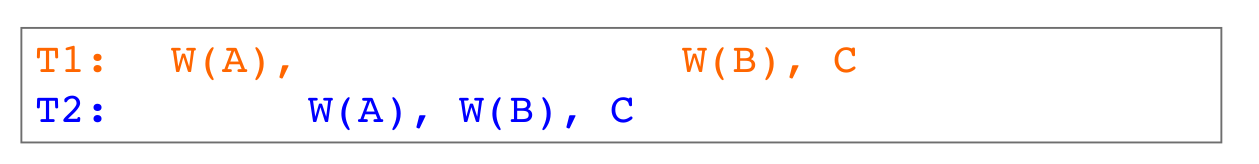
\includegraphics[scale=0.15]{graphics/WW-conflicts.png}

\end{itemize}

% LocalWords:  Atomicity atomicity modularity Serializability Xacts
% LocalWords:  TODO priori Xact systems's Serializable WR RW
